\documentclass[11pt]{article}
\usepackage{fullpage,amsmath,graphicx}

% --- -----------------------------------------------------------------
% --- Document-specific definitions.
% --- -----------------------------------------------------------------
\newtheorem{definition}{Definition}

\newcommand{\concat}{{\,\|\,}}
\newcommand{\bits}{\{0,1\}}

% --- -----------------------------------------------------------------
% --- The document starts here.
% --- -----------------------------------------------------------------
\begin{document}
\sloppy

\noindent Rutgers University\\
CS440: Introduction to Artificial Intelligence, Spring 2017\\
Kostas Bekris\\

\begin{center}
\LARGE{\textbf{Homework 4: James Carroll and Joel Carrillo}}\\
\large{\textbf{\emph{Decision Making under Uncertainty and Learning}}}
\end{center}

\vspace{.1in}

\begin{enumerate}

\item Question 1
\begin{enumerate}
\item Starting with an arbitrary discount of 0.4 and values (0, 0, 0, 0), it took one millisecond and five iterations to find the optimal policy of: Action 2 at State 1; Action 2 at State 2; Action 3 at State 3; and Action 1 at State 4. \\ \\
The optimal utility at the respective states are 0.14690304000000004, 0.39942144000000007, 1.1707264, and 0.43098624000000013. The method was repeatedly applying the Bellman equation to find the policy that maximizes the utility function. Intermediate values:
\begin{enumerate}
\item Policy [0, 0, 0, 0] Values [0, 0, 1, 0]
\item Policy [0, 0, 0, 0] Values [0, 0.32, 1, 0.36]
\item Policy [0, 1, 0, 0] Values [0.1152, 0.3456, 0.144, 0.3744]
\item Policy [1, 1, 2, 0]  Values [0.129024, 0.393728, 1.14976, 0.426816]
\item Policy [1, 1, 2, 0]  Values [0.14690304, 0.39942144, 1.1707264, 0.43098624]
\end{enumerate}
\end{enumerate}
\item Question 2
\begin{enumerate}
\item Yes.
\item Gain(GPA) = $I(\frac{p}{p+n}, \frac{n}{p+n})$ - Remainder(GPA) \\
$I(\frac{6}{6+6}, \frac{6}{6+6}) = I(\frac{1}{2}, \frac{1}{2}) = 1$ \\
Gain(GPA) = 1 - $\sum_{i=1}^{v} \frac{p_i + n_i}{p + n} I(\frac{p_i}{p_i + n_i},\frac{n_i}{p_i + n_i}) $ \\
Gain(GPA) = 1 - $[\frac{4}{12} I(0,1) + \frac{5}{12} I(\frac{3}{5}, \frac{2}{5}) + \frac{3}{12} I(1, 0)]$ \\
Gain(GPA) = 1 - $\frac{4}{12} * 0 + \frac{5}{12} * (0.9710) + \frac{3}{12} * 0 = 0.5954$ \\
Gain (Pub) = 1 - $[\frac{7}{12} I(\frac{3}{7}, \frac{4}{7}) + \frac{5}{12} I(\frac{3}{5}, \frac{2}{5}))] = 0.0207$ \\
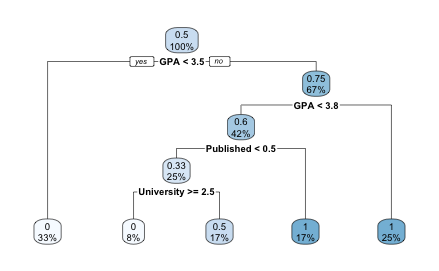
\includegraphics[scale=0.5]{gpaplot}
\item Yes, because the information gain for GPA is highest, Publications is second-highest, and so forth.
\end{enumerate}
\item Question 3
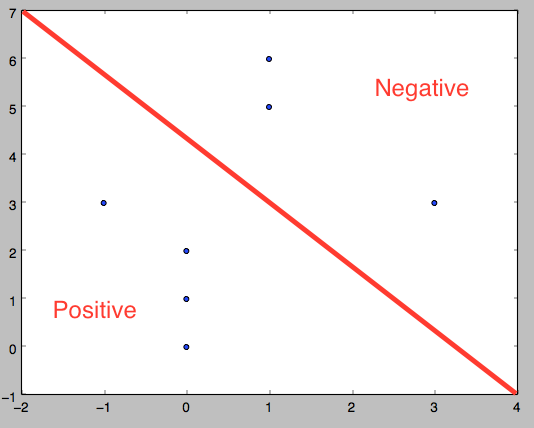
\includegraphics[scale=0.5]{svm}
\item Question 4
\item Question 5

\end{enumerate}
\end{document}
